%-------------------------
% Resume in Latex
% Author: Huirem Nikhil Singh (Ece 2020 - 2024)
% License : MIT
%------------------------

%---- Required Packages and Functions ----

\documentclass[a4paper,11pt]{article}
\usepackage{latexsym}
\usepackage{xcolor}
\usepackage{float}
\usepackage{ragged2e}
\usepackage[empty]{fullpage}
\usepackage{wrapfig}
\usepackage{lipsum}
\usepackage{tabularx}
\usepackage{titlesec}
\usepackage{geometry}
\usepackage{marvosym}
\usepackage{verbatim}
\usepackage{enumitem}
\usepackage[hidelinks]{hyperref}
\usepackage{fancyhdr}
\usepackage{fontawesome5}
\usepackage{multicol}
\usepackage{graphicx}
\usepackage{cfr-lm}
\usepackage[T1]{fontenc}
\setlength{\multicolsep}{0pt} 
\pagestyle{fancy}
\fancyhf{} % clear all header and footer fields
\fancyfoot{}
\renewcommand{\headrulewidth}{0pt}
\renewcommand{\footrulewidth}{0pt}
\geometry{left=1.4cm, top=0.8cm, right=1.2cm, bottom=1cm}
% Adjust margins
%\addtolength{\oddsidemargin}{-0.5in}
%\addtolength{\evensidemargin}{-0.5in}
%\addtolength{\textwidth}{1in}
\usepackage[most]{tcolorbox}
\tcbset{
	frame code={}
	center title,
	left=0pt,
	right=0pt,
	top=0pt,
	bottom=0pt,
	colback=gray!20,
	colframe=white,
	width=\dimexpr\textwidth\relax,
	enlarge left by=-2mm,
	boxsep=4pt,
	arc=0pt,outer arc=0pt,
}

\urlstyle{same}

\raggedright
\setlength{\tabcolsep}{0in}

% Sections formatting
\titleformat{\section}{
  \vspace{-4pt}\scshape\raggedright\large
}{}{0em}{}[\color{black}\titlerule \vspace{-7pt}]

%-------------------------
% Custom commands
\newcommand{\resumeItem}[2]{
  \item{
    \textbf{#1}{\hspace{0.5mm}#2 \vspace{-0.5mm}}
  }
}

\newcommand{\resumePOR}[3]{
\vspace{0.5mm}\item
    \begin{tabular*}{0.97\textwidth}[t]{l@{\extracolsep{\fill}}r}
        \textbf{#1}\hspace{0.3mm}#2 & \textit{\small{#3}} 
    \end{tabular*}
    \vspace{-2mm}
}

\newcommand{\resumeSubheading}[4]{
\vspace{0.5mm}\item
    \begin{tabular*}{0.98\textwidth}[t]{l@{\extracolsep{\fill}}r}
        \textbf{#1} & \textit{\footnotesize{#4}} \\
        \textit{\footnotesize{#3}} &  \footnotesize{#2}\\
    \end{tabular*}
    \vspace{-2.4mm}
}

\newcommand{\resumeProject}[4]{
\vspace{0.5mm}\item
    \begin{tabular*}{0.98\textwidth}[t]{l@{\extracolsep{\fill}}r}
        \textbf{#1} & \textit{\footnotesize{#3}} \\
        \footnotesize{\textit{#2}} & \footnotesize{#4}
    \end{tabular*}
    \vspace{-2.4mm}
}

\newcommand{\resumeSubItem}[2]{\resumeItem{#1}{#2}\vspace{-4pt}}

% \renewcommand{\labelitemii}{$\circ$}
\renewcommand{\labelitemi}{$\vcenter{\hbox{\tiny$\bullet$}}$}

\newcommand{\resumeSubHeadingListStart}{\begin{itemize}[leftmargin=*,labelsep=0mm]}
\newcommand{\resumeHeadingSkillStart}{\begin{itemize}[leftmargin=*,itemsep=1.7mm, rightmargin=2ex]}
\newcommand{\resumeItemListStart}{\begin{justify}\begin{itemize}[leftmargin=3ex, rightmargin=2ex, noitemsep,labelsep=1.2mm,itemsep=0mm]\small}

\newcommand{\resumeSubHeadingListEnd}{\end{itemize}\vspace{2mm}}
\newcommand{\resumeHeadingSkillEnd}{\end{itemize}\vspace{-2mm}}
\newcommand{\resumeItemListEnd}{\end{itemize}\end{justify}\vspace{-2mm}}
\newcommand{\cvsection}[1]{%
\vspace{2mm}
\begin{tcolorbox}
    \textbf{\large #1}
\end{tcolorbox}
    \vspace{-4mm}
}

\newcolumntype{L}{>{\raggedright\arraybackslash}X}%
\newcolumntype{R}{>{\raggedleft\arraybackslash}X}%
\newcolumntype{C}{>{\centering\arraybackslash}X}%
%---- End of Packages and Functions ------

%-------------------------------------------
%%%%%%  CV STARTS HERE  %%%%%%%%%%%
%%%%%% DEFINE ELEMENTS HERE %%%%%%%
\newcommand{\name}{WenChao Li} % Your Name
\newcommand{\sex}{Male} % Your sex
\newcommand{\from}{Beijing, China} % your country
\newcommand{\School}{Studying for a PhD at Beihang University} % Your School
\newcommand{\phone}{13261883805} % Your Phone Number
\newcommand{\emaila}{liwenchao55@126.com} %Email 1
\newcommand{\emailb}{wenchaoli@buaa.edu.cn} %Email 2




\begin{document}
\fontfamily{cmr}\selectfont
%----------HEADING-----------------


\parbox{2.35cm}{%
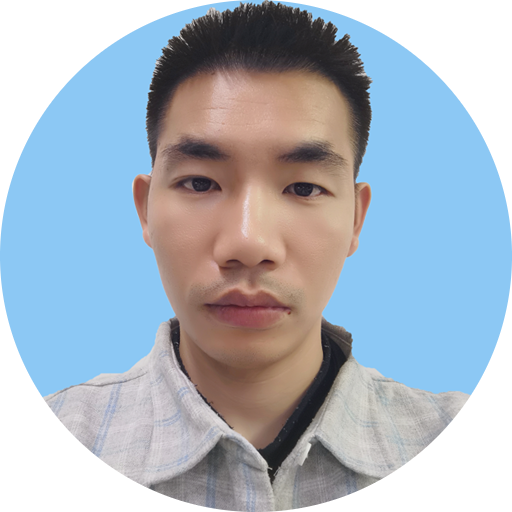
\includegraphics[width=2.35cm,clip]{wenchaoli.png}}
\parbox{\dimexpr\linewidth-2.8cm\relax}{
\begin{tabularx}{\linewidth}{L r} \\
  \textbf{\Large \name} & {\raisebox{0.0\height}{\footnotesize \faPhone}\ \phone}\\
  {Sex: \sex} & \href{mailto:\emaila}{\raisebox{0.0\height}{\footnotesize \faEnvelope}\ {\emaila}} \\
  \from &  \href{mailto:\emailb}{\raisebox{0.0\height}{\footnotesize \faEnvelope}\ {\emailb}}\\
  \School &  \href{https://liwenchao0615.github.io/WenChaoLi1108.github.io/}{\raisebox{0.0\height}{\footnotesize \faGithub}\ {Personal homepage}} \\
  {Targeted Detection, Image Recovery, Computer Vision} &  \href{https://scholar.google.com/citations?user=ph9tt1oAAAAJ\&hl=en}{\raisebox{0.0\height}{\footnotesize \faGraduationCap} {Google Scholar Profile}}
\\


\end{tabularx}
}
% \parbox{3.0cm}{%
% \flushright \includegraphics[width=2cm,clip]{nitp_logo.png}
% }


%-----------EDUCATION-----------
\section{\textbf{Education}}
  \resumeSubHeadingListStart
    \resumeSubheading
      {Beihang University} {Ph.D.}
      {Measuring and Testing Technologies and Instruments}{2021,09-Now}
    \resumeSubheading
      {Nanchang Hangkong University}{M.S.}
      {Measuring and Testing Technologies and Instruments}{2018,09-2021,06}
    \resumeSubheading
      {Nanchang Hangkong University}{B.S.}
      {Measurement and Control Technology and Instrumentation}{2014,09-2018,06}
  \resumeSubHeadingListEnd
\vspace{-5.5mm}
%



%-----------EXPERIENCE-----------------
\section{\textbf{Experience}}
  \resumeSubHeadingListStart
    \resumeSubheading
      {Helicopter Design and Research Institute}{Jingdezhen, China}
      {(Project Manager)}{2022,05-2022,06}
      \vspace{-2.0mm}
      \resumeItemListStart
    \item {Acquisition of outdoor helicopter rotor blade flight parameters for the Iron Bird Terrace}
    \item {QT Interface Development}
    \resumeItemListEnd
    
    \vspace{-3.0mm}
    
    \resumeSubheading
      {Jingdong Exploration Research Institute}{Beijing, China }
      {(Research Assistant)}{2021,12-2022,01}
      \vspace{-2.0mm}
      \resumeItemListStart
    \item {Target detection in complex scenes}
    \item {Object Rotation Target Detection in Complex Scenes}
    \resumeItemListEnd
      
  \resumeSubHeadingListEnd
\vspace{-8.5mm}



%-----------Published Papers-----------------
\section{\textbf{Published Papers}}

{\faIcon{book-open} \textbf{Conference and journal papers} \hfill   first author} %Project Name
\vspace{10pt} % 添加垂直间距
\begin{itemize}
  \item RT-Net: A Real-time Detection Network for helicopterRotor-tail
  \vspace{10pt} % 添加垂直间距
  \item Zero-Shot Enhancement of Low-Light Image Based on Retinex Decomposition
  \vspace{10pt} % 添加垂直间距
  \item Numerical investigations of ultrasonic reverse time migration for complex cracks near the surface
\end{itemize}


%-----------Technical skills-----------------
\section{\textbf{Technical Skills and Interests}}
\vspace{10pt} % 添加垂直间距
 \begin{itemize}[leftmargin=0.05in, label={}]
    \small{\item{
     \textbf{Developer Tools}{: Python, C/C++, C\#, Java,  Matlab, Git, Scripting (Bash), LaTeX, HTML, Vim} \\
     \vspace{10pt} % 添加垂直间距
     \textbf{Frameworks}{: Linux, Tensorflow, Pytorch, Docker, OpenCV, Solidworks, Unity Engine } \\
     \vspace{10pt} % 添加垂直间距
     \textbf{Areas of Interest}{: Computer vision, multimodal, smart hardware, robotics development, drone development} \\
     \vspace{10pt} % 添加垂直间距
    }}
 \end{itemize}
 \vspace{-16pt}



%-----------Positions of Responsibility-----------------
\section{\textbf{Positions of Responsibility}}
\vspace{-0.4mm}
\resumeSubHeadingListStart
\resumePOR{Founding Member, } % Position
    {Beihang Leadership Club} %Club,Event
    {Permanent Member} %Tenure Period
\resumePOR{Student Membership, } % Position
    {Chinese Society of Image and Graphics} %Club,Event
    {four-year} %Tenure Period
\resumeSubHeadingListEnd
\vspace{-5mm}




%-----------personal account-----------------
\section{\textbf{personal account}}
\vspace{10pt}
I am very passionate about research and feel a sense of accomplishment when I am solving a problem. My areas of interest include visual detection in complex scenes, image reconstruction and restoration, multimodal detection tasks, and intelligent hardware devices, and I like to pair advanced deep learning theories with hardware devices to solve the challenges that people encounter in real life.

I am a self-motivated person, I can complete the tasks assigned by my boss quickly, and I am capable of both software and hardware development. I hope to join the lab, contribute to the lab construction, and work together to accomplish interesting research.
\vspace{-5mm}



%-------------------------------------------
\end{document}
